% \renewcommand{\thefigure}{A.\arabic{section}.\arabic{figure}hhh}
\counterwithin{figure}{section}
\setcounter{section}{3} % Assuming section A.3 corresponds to section 3
\setcounter{figure}{0}  % Reset figure counter for this section


%%%%%%%%%%%%%%%%%%%%
%% SUPPLEMENTARY %%%
%%%%%%%%%%%%%%%%%%%%

\begin{figure}[htbp]
  \centering
  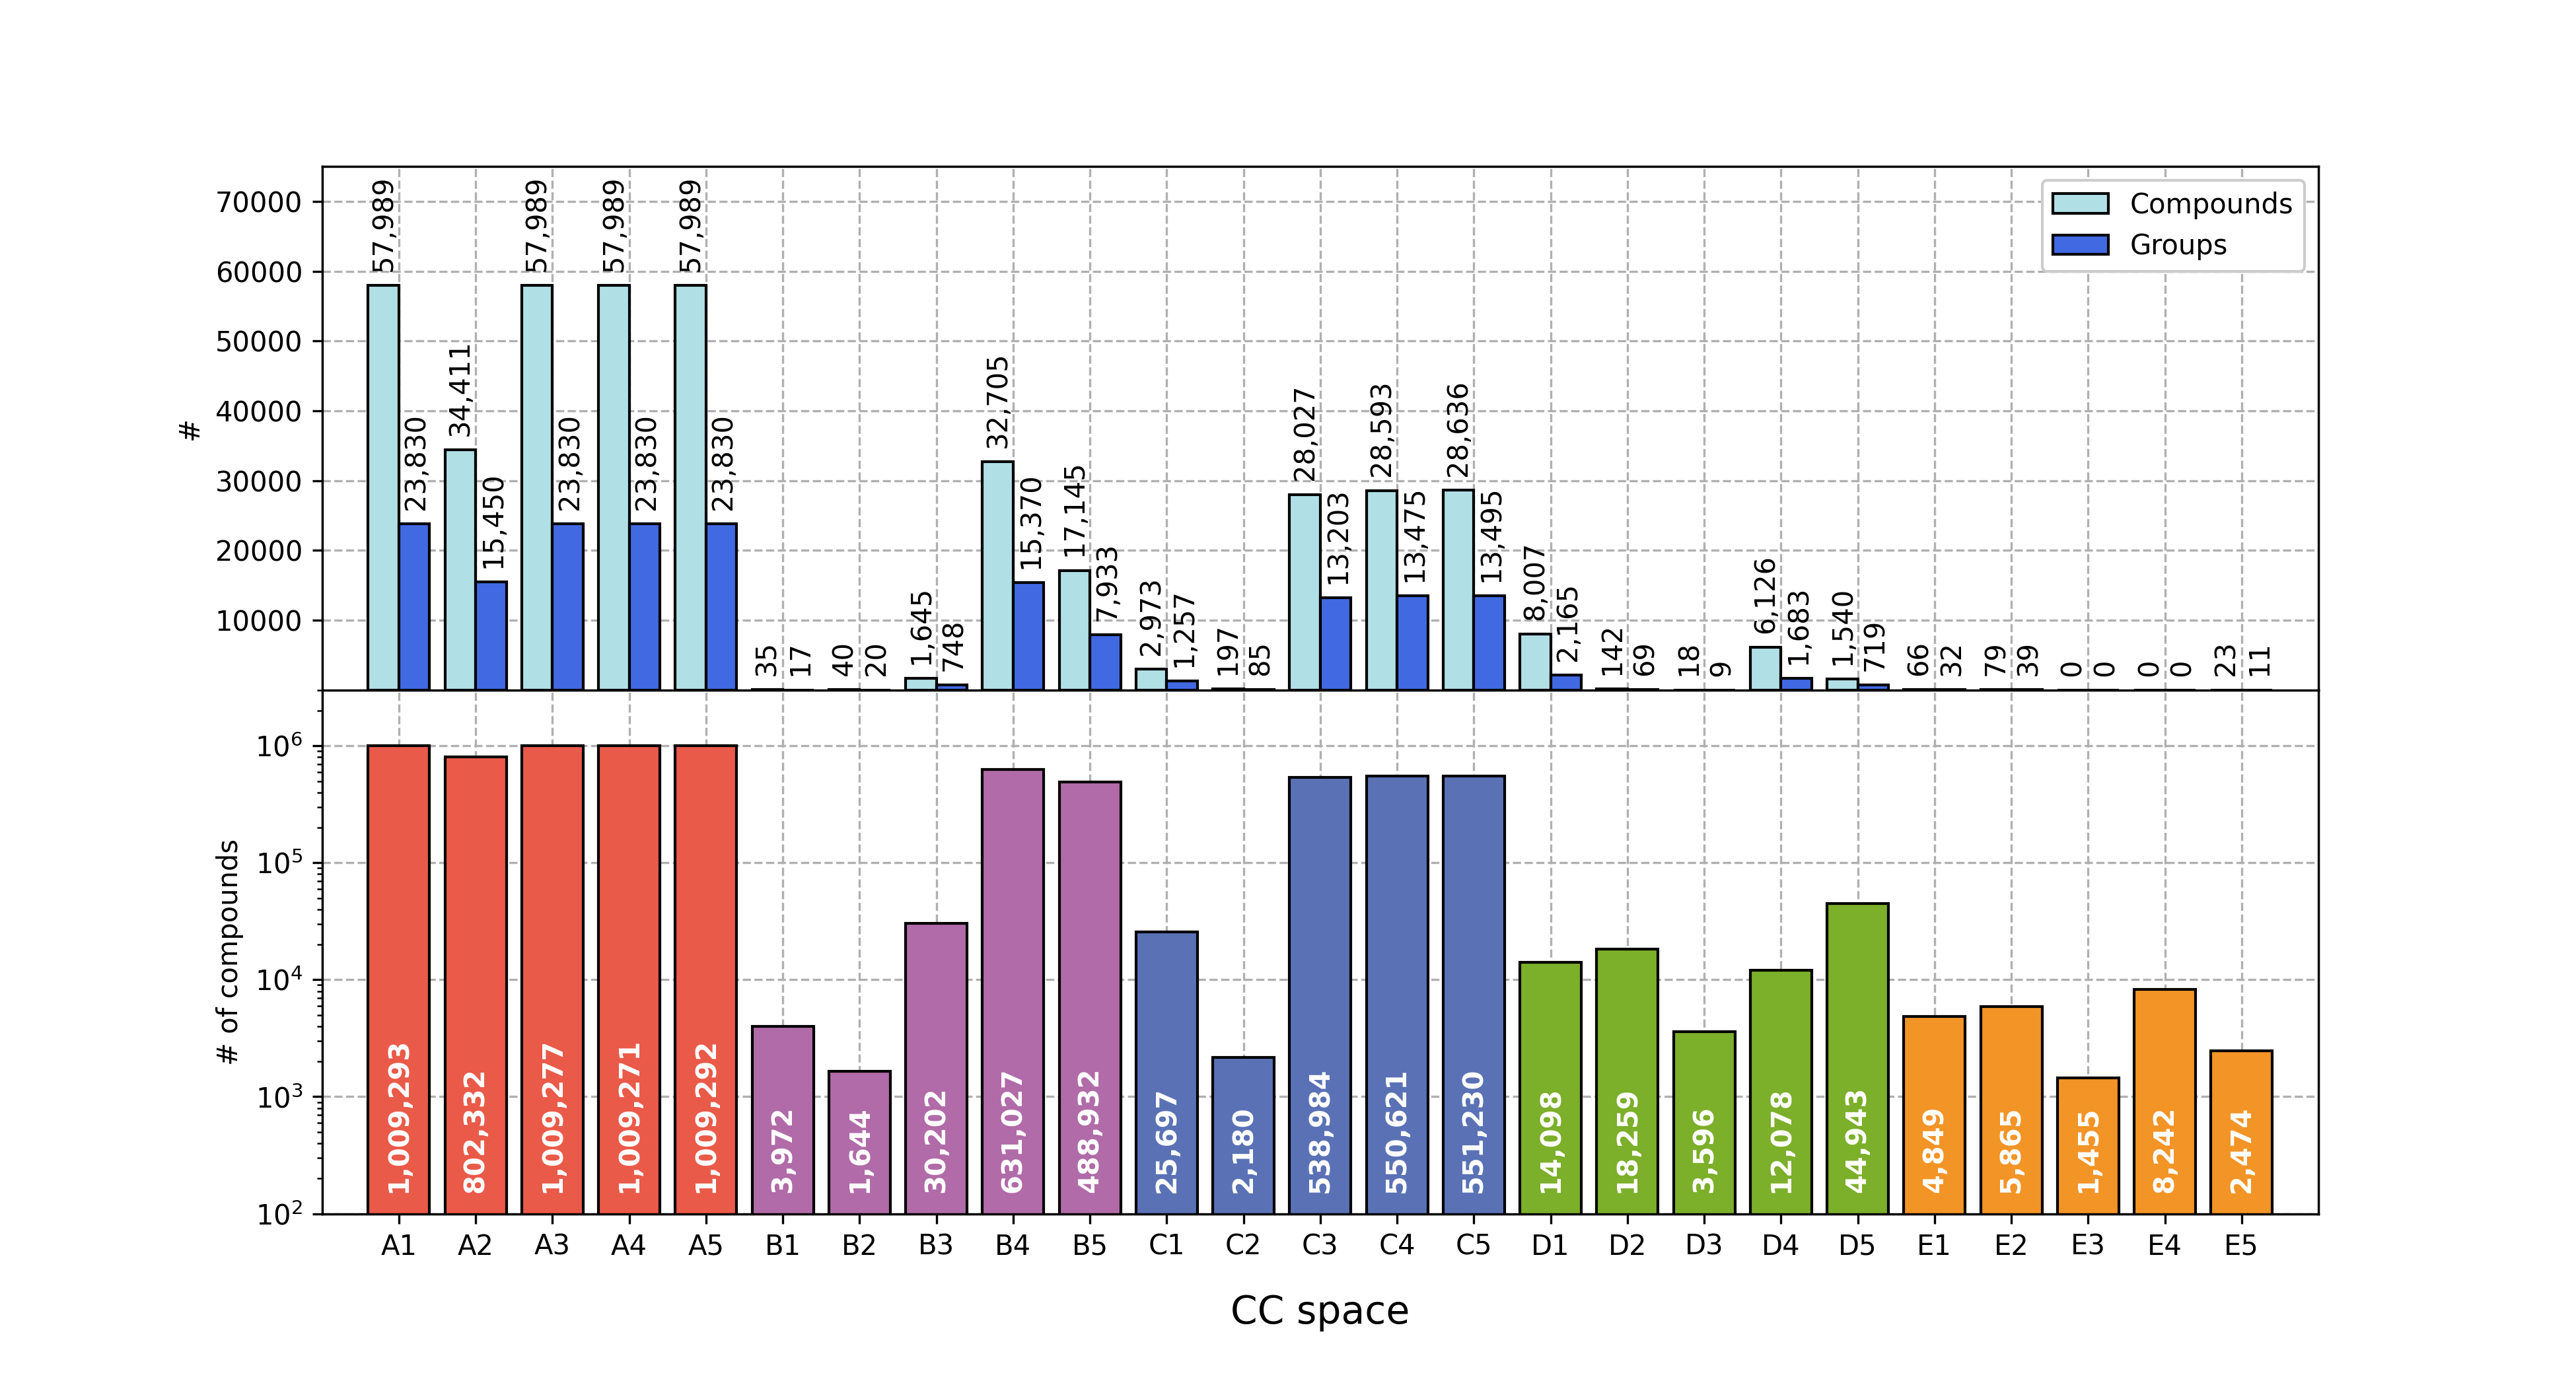
\includegraphics[width=1\linewidth]{figures/Stereoisomers/Supplementary/FigS1.png}
  \caption{Number of compounds (bottom) in each CC space. Number of groups of stereoisomers and number of stereoisomers (top) in each CC space.}
  \label{Stereoisomers_FigS1}
\end{figure}



\begin{figure}[htbp]
  \centering
  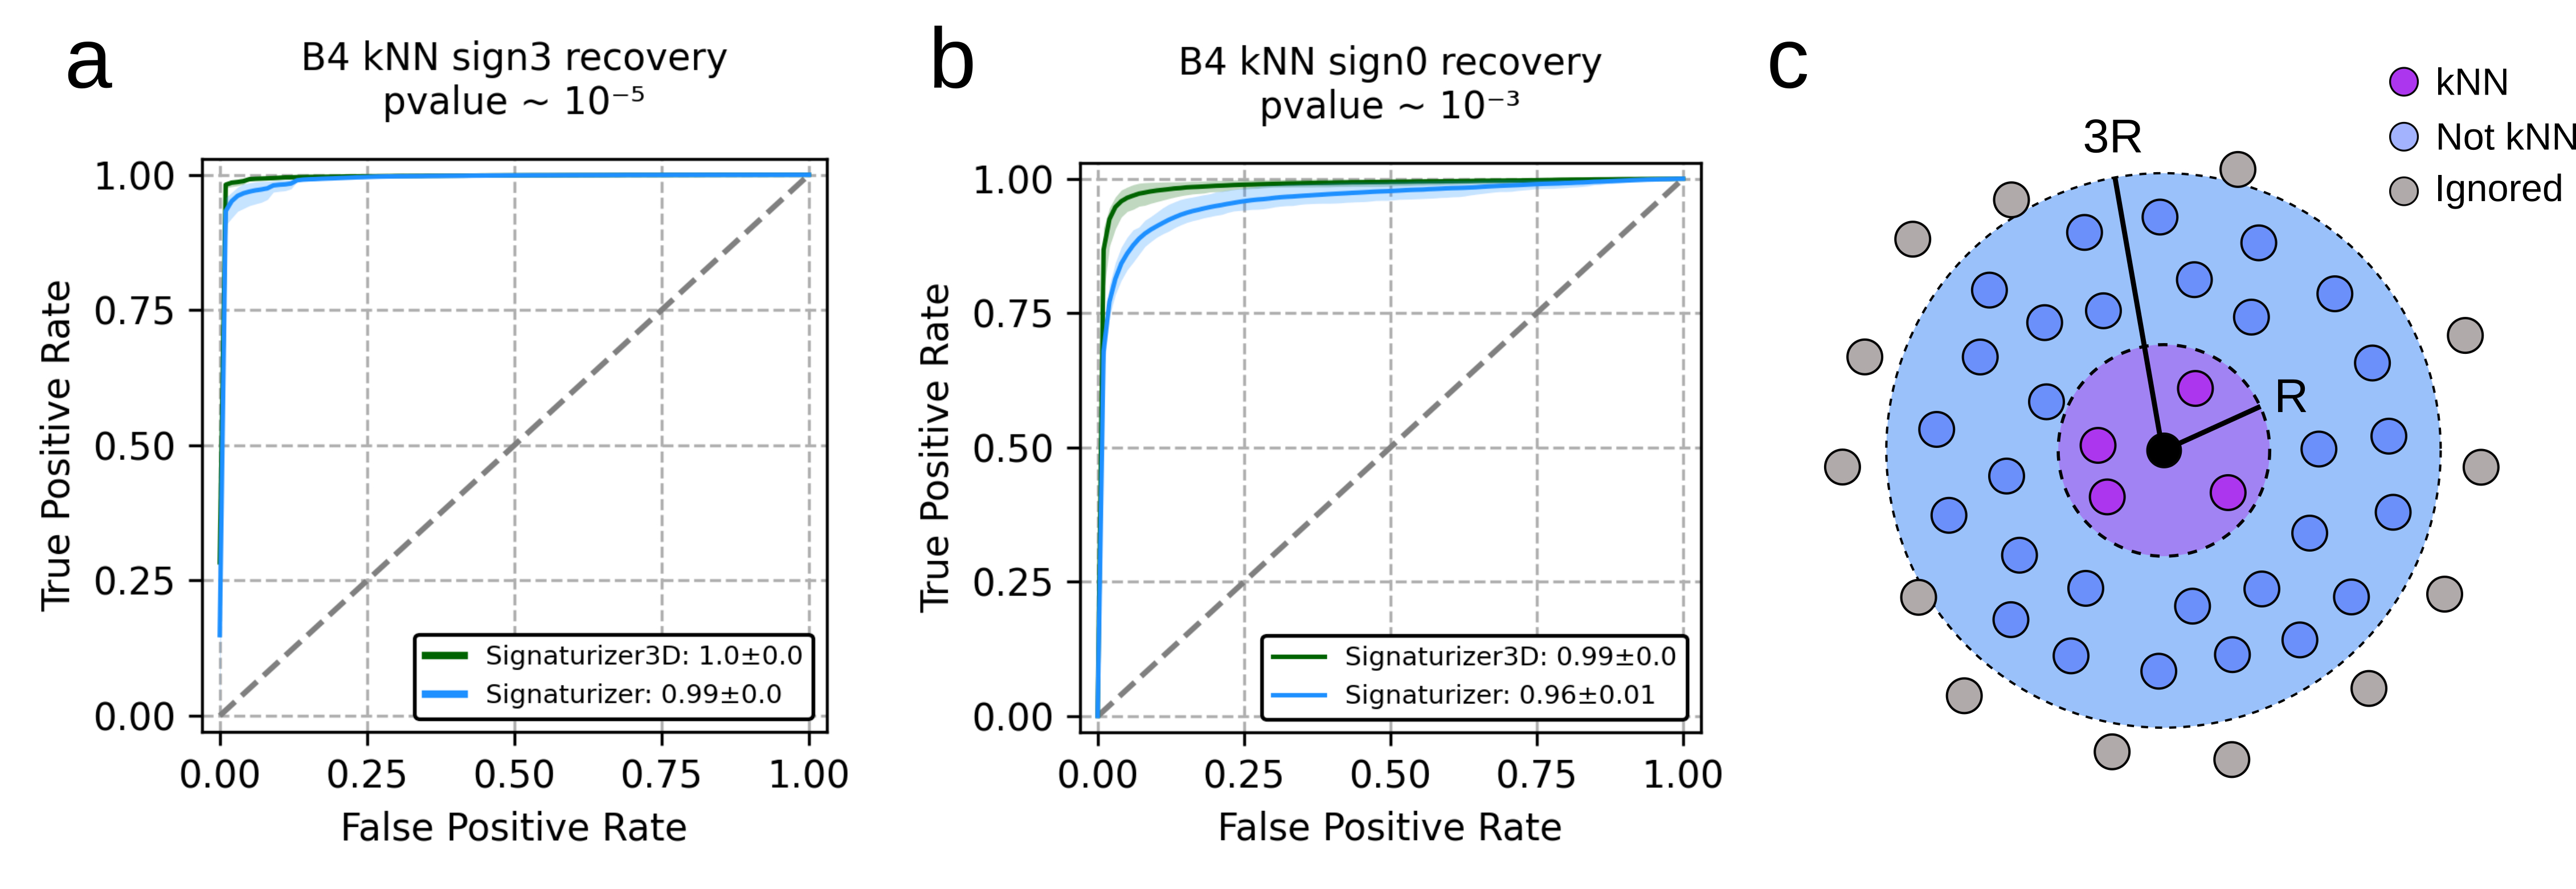
\includegraphics[width=1\linewidth]{figures/Stereoisomers/Supplementary/FigS2.png}
  \caption{
    \textbf{a)} Recapitulation of B4 signature type III kNNs (x3 80/20 splits) using the original Signaturizer and the Signaturizer3D. Nearest neighbors were defined as those molecules with a B4 cosine distance to the evaluated compound in the 0.001 percentile of the distribution (p-value \textasciitilde10\textsuperscript{-5}).
    \textbf{b)} Recapitulation of B4 signature type 0 kNNs using the original Signaturizer and the Signaturizer3D. Nearest neighbors were defined as those molecules with a B4 cosine distance to the evaluated compound in the 0.1 percentile of the distribution (p-value \textasciitilde10\textsuperscript{-3}).
    \textbf{c)} Stringent strategy to assess the recovery of k nearest neighbors (kNN): given a seed compound (black), NNs are defined as those k compounds being at a distance <R (purple). On the other hand, non-NN are defined as those compounds being at a distance >R but <3R (blue), so that non-NN are still close to the real neighbors. All compounds at a distance >3R (gray) are ignored. The R was set to the 0.001 (pvalue \textasciitilde10\textsuperscript{-5}) and 0.1 (pvalue \textasciitilde10\textsuperscript{-3}) percentile of closest compounds for type III and 0 signatures, respectively, which reflect the different number of compounds and possible comparisons in each space.
  }
  \label{Stereoisomers_FigS2}
\end{figure}